\documentclass{report}
\usepackage{fullpage}
\usepackage{graphicx}
\begin{document}
\title{Savant Genome Browser: Developer Manual}
\maketitle

\setlength{\parindent}{0pt} 
\setlength{\parskip}{2ex}

Author: Marc Fiume \\
Contact: savant@cs.toronto.edu \\
Website: http://compbio.cs.toronto.edu/savant/ \\
\\
This document applies to Savant version 1.02\\

\newpage

\tableofcontents

\newpage

\chapter{Introduction}

\section{What is Savant Development?}

Savant was designed to be accessible and extensible. This means that third-party tools can be developed to create tracks which are immediately loadable in Savant and do not need formatting (e.g. from some upstream analysis program) or to extend the browser (e.g. to perform realtime custom analyses) via a plugin.

\section{Who should develop for Savant and why?}

Existing genome browsers are limited in functionality and do not afford the necessary means to efficiently perform tasks required by their users. Savant provides core functionalities found in popular genome browsers like UCSC, and it can be further extended to enable custom tasks. Savant's extensibility makes it a powerful platform on which to develop novel functionalities, including custom visualizations and analyses.

Savant files can be created using virtually any programming language (e.g. C, C++, Python, etc.). Developers interested in creating a plugin should be familiar with the Java Programming Language. 

\chapter{Savant Code}

\section{Implementation}

Savant is implemented in the {\bf Java Programming Language}, since the language is easy to learn and runs on all major platforms. Plugins must also be implemented in Java.

\section{Organization}

Savant is designed under the {\bf Model-View-Controller software engineering paradigm}. That is, the code which governs input and presentation elements (UI and visualization, respectively) is isolated from the application logic (data reading, writing, and manipulation).

\begin{figure*}[!h]
\begin{center}
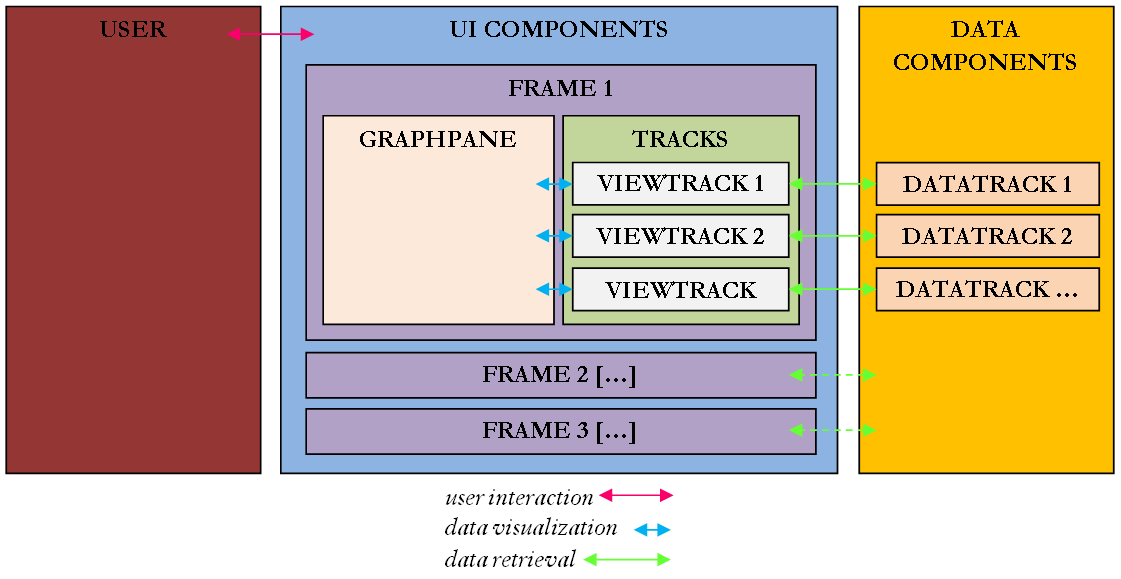
\includegraphics[type=png,ext=.png,read=.png,width=16cm]{images/arch}
\caption{Schematic of the Savant code architecture}
\label{}
\end{center}
\end{figure*}

\subsection{UI Components}

The UI Components are involved in receiving and responding to user input, in addition to visualizing data.

\begin{itemize}
\item{} {\bf Frame} A frame is a container for visualizing one or more tracks. Each frame contains its own Graphpane. Each frame is also associated with one or more Tracks.
\item{} {\bf Graphpane} A Graphpane is a canvas for drawing. Data is visualized on the graphpane, as well as other features such as gridlines and legends.
\item{} {\bf Track} A Track is a lens into a track. It communicates with a DataSource and delegates a renderer to draw the received data.
\end{itemize}

\subsection{Data Components}

The Data Components are involved reading data from track files as requested by its corresponding Track.

\begin{itemize}
\item{} {\bf DataSource} A DataSource retrieves data from a track file in a specified range, usually requested by the Track upon a user's changing of the range. There is a DataSource specific for each file type, since the file structures for the various track types differ.
\end{itemize}

\chapter{Plugin Development}

\section{Plugin Framework}

Savant uses the Java Plugin Framework (JPF) as its plugin framework. See http://jpf.sourceforge.net/ for detailed documentation on JPF.

\section{Developing a plugin}

\subsection{The Plugin SDK}

To begin developing a custom plugin, download the Savant SDK from the Savant website (http://compbio.cs.toronto.edu/savant/) and expand it. The following directories and files are included:
\begin{itemize}
\item{} {\bf doc} Contains documentation, including a copy of this developer guide and JavaDoc API documentation for Savant.
\item{} {\bf lib} Contains external libraries used by Savant that a plugin may require. 
\item{} {\bf log4j.properties} A basic log4j.properties file to provide debugging output to the console.This can be edited. (See Debugging section below)
\item{} {\bf plugins} Contains plugins to be loaded when Savant is run, including the required SavantCore.jar plugin. To test a plugin, it must be deplyed here. (See Building and Deploying the Plugin below.)
\item{} {\bf runWithLog.sh} A shell script for Unix and Mac OS X to run Savant with Log4J logging configured for debugging. (See Debugging section below)
\item {\bf SavantPluginSample} A sample plugin project. Contains source code for the sample plugin, plus a NetBeans project that can be used to examine and build it.
\item {\bf SavantSDK.jar} Along with the contents of the lib directory, a plugin project will need this .jar file on its classpath.
\end{itemize}

\subsection{Setting the Classpath}

As mentioned above, a new plugin project will require some additions to its classpath. Specifically, the SavantSDK.jar and lib/jpf.jar files are required by all plugins. Other entries in the lib directory may be required, depending on what functionality the plugin implements. For logging, lib/commons-logging-1.1.1.jar and lib/log4j.jar will also be necessary. For plugins which require access to BAM alignment maps, the lib/sam-1.12.jar file will need to be added, and so on.

\subsection{Creating the Plugin Class}

The following is a complete implementation of a plugin.

\begin{verbatim}
public class DataTab extends Plugin implements AuxData {

     public void init(JTabbedPane tabbedPane, PluginAdapter pluginAdapter) {
        JPanel tablePanel = createTabPanel(tabbedPane, "Data View");
        DataSheet currentRangeDataSheet = new DataSheet(tablePanel, pluginAdapter);
        pluginAdapter.getRangeController().
            addRangeChangedListener(currentRangeDataSheet);
        pluginAdapter.getTrackController().
            addTracksChangedListener(currentRangeDataSheet);
    {
    

    private JPanel createTabPanel(JTabbedPane jtp, String name) {
        JPanel pan = new JPanel();
        pan.setLayout(new BorderLayout());
        pan.setBackground(BrowserDefaults.colorTabBackground);
        jtp.addTab(name, pan);
        return pan;
    }

    @Override
    protected void doStart() throws Exception {}

    @Override
    protected void doStop() throws Exception {}

}
\end{verbatim}    

The plugin implementation class must extend org.java.plugin.Plugin. This requires it to override two abstract methods: doStart() and doStop(). In both cases, the implementations must be empty. (See http://jpf.sourceforge.net/ for details.)

In addition, the plugin implementation must implement the interface savant.plugin.AuxData. AuxData is the only plugin interface currently available to Savant plugins. It contains a single method, init(), which is called by Savant after the plugin has been loaded. All the code required to initialize the plugin and its interface (if any) must be done here. 

The init() method is passed two arguments: an instance of javax.swing.JTabbedPane and an instance of savant.plugin.PluginAdapter. The former provides a Swing pane in which the plugin can create a UI. The latter provides some convenience methods for the plugin's use, e.g. getRangeController() and getTrackController(). For a complete list of methods provided and their usage, consult the most recent JavaDoc documentation.

\subsection{Plugin Descriptor}

In addition to Java source code, a plugin must provide a plugin descriptor file called plugin.xml that describes the plugin to the Savant plugin framework. The following descriptor file describes the sample plugin:

\begin{verbatim}
<?xml version="1.0" ?>
<!DOCTYPE plugin PUBLIC "-//JPF//Java Plug-in Manifest 1.0" 
    "http://jpf.sourceforge.net/plugin_1_0.dtd">
<plugin id="savant.data" version="1.0.0"
    class="savant.data.DataTab">
<requires><import plugin-id="savant.core"/></requires>
    <runtime>
        <library id="data" path="/" type="code">
            <export prefix="*" />
        </library>
    </runtime>
    <extension plugin-id="savant.core" point-id="AuxData" id="DataTab">
        <parameter id="class" value="savant.data.DataTab"/>
        <parameter id="name" value="Data"/>
    </extension>
</plugin>
\end{verbatim} 

The {\bf plugin} element takes a unique id attribute and the fully-qualified class name of the Plugin extension class in its id attribute.

The {\bf requires} element imports the savant.core plugin, which is the plugin which provides the extension points for all other Savant plugins.

The {\bf runtime} element specifies that all packages in the plugin will be exported for use by other plugins.

Finally, the {\bf extension} element defines the extended plugin in its plugin-id attribute. As previously discussed, all Savant plugins extend savant.core. The point-id attribute refers to the extension point, and as previously discussed the only existing extension point is AuxData. The id attribute simply requires a unique id. The two nested {\bf parameter} elements declare the fully-qualified class name (again) and a name parameter which is used as the JTabbedPane title for the tab.

\subsection{Building and Deploying the Plugin}

A plugin is deployed as a .jar file containing all of the classes required by the plugin as well as the plugin.xml descriptor file. This .jar file is placed in the plugins directory of Savant. When Savant is (re)started, it loads all plugins contained in the plugins directory.

If a plugin depends on any third-party classes or libraries, these must be exploded and included in the plugin's .jar file. In other words, the .jar file must contain all resources required by the plugin.

\subsection{Debugging}

The Savant SDK provides the capability to test a plugin without interfering with an installed version of the application. The compiled and packaged plugin may be placed in the {\bf plugins} folder of the Savant SDK. Double-clicking on SavantSDK.jar will run the application with the plugin loaded. If desired, a debugger may be attached to the local process for detailed debugging of the plugin. 

Using the runWithLog.sh script will load the log4j.properties file and create logging output accordingly. By default, logging output goes to the Unix console. For use on Windows, a FileAppender may be required. A plugin class can make use of logging by creating a logger and calling its methods, e.g.:

\begin{verbatim}
import org.apache.commons.logging.Log;
import org.apache.commons.logging.LogFactory;

public class DataTab extends Plugin implements AuxData {

    private static Log log = LogFactory.getLog(DataTab.class);

    //  ...
    log.info("Info message");
    log.debug("Debug message");
    // etc.
}
\end{verbatim}

\chapter{Generating Savant Files}

\section{Savant File Format}

Savant files are written in a highly structured binary format so as to maximize the speed of data retrieval. Since BAM files are already stored in a fashion which permits fast retrieval, no formatting of these files is necessary and they can be loaded directly into Savant.

\subsection{Version}

This document outlines {\bf Version 1} of the the format specifications. Files formatted with this specification are (at least) compatible with Savant 1.02.

\subsection{Endian-ness}

Savant only reads and writes files in {\bf big-endian byte order}. This is the default byte order of output streams in Java. In the case in which upstream programs cannot be modified to output files in big-endian byte order, it is recommended to use text output and simply format them using the provided Savant formatting tools.

\subsection{File Structure}

Savant files are stored in two parts:

\begin{itemize}
\item{} {\bf Header} Identifies a file as a Savant file, its type, and other type-specific information such as field names and lengths.
\item{} {\bf Body} Contains a listing of records (e.g. SNP records, or gene records).
\end{itemize}

\subsubsection{File Header}

The file header for a Savant file contains the following in order:

\begin{itemize}
\item{} {\bf Savant File Identifier} A Savant file is identified through a {\bf magic number}. The magic number is comprised of {\it exactly} 4 bytes. The first three bytes must be: FA, CE, and BE. The fourth byte must correspond to the type of track that the file represents, as specified in Table \ref{bytetable}.

\begin{table}[h] 
\caption{Last Byte in Magic Number for All Savant File Types}  
\begin{tabular*}{6in}{ l l }  
\hline                      
Savant File Type & Last Byte \\
\hline                    
Generic Interval formatted for Savant & 03 \\
BED formatted for Savant & 04 \\
GFF formatted for Savant & 05 \\
WIG formatted for Savant & 06 \\
Continuous Generic formatted for Savant & 07 \\
FASTA formatted for Savant &  08 \\
Generic Point formatted for Savant & 09 \\
\hline     
\label{bytetable}
\end{tabular*} 
\end{table} 

\item{} {\bf Version} A number corresponding to the version of the {\it format specifications} used to create the file.

\item{} {\bf Filetype-specific information} Additional information is provided, depending on the filetype:

\subitem{Generic Point}: Write [FieldType.INTEGER] and [FieldType.STRING] in that order
\subitem{Generic Continuous}: Write [FieldType.FLOAT]
\end{itemize}

Notes:
\begin{itemize}
\item{} No additional information is written for Sequence Tracks.
\item{} The FieldType enum can be found in the source code of Savant. The integer representing [FieldType.INTEGER], for example, is the 0-based index that INTEGER appears in the FieldType enum list in FieldType.java.
\end{itemize}

\subsubsection{File Body}

The bodies of Savant files are composed of consecutive {\bf fixed-length records}. The bodies are therefor of the form:
\begin{verbatim}
	[record 1]
	[record 2]
	[record ...]
	[record N]
\end{verbatim}

{\it Records in Sequence Files} Each record in a sequence file is a single character, where the ith character in the body corresponds to the ith character in the sequence.

\begin{verbatim}
	[record] = [char: a nucleotide letter]
\end{verbatim}

{\it Records in Point Files} Each record in a point file is a single float, where the ith float in the body corresponds to the value at ith position.

\begin{verbatim}
	[record] = [float: a value]
\end{verbatim}

{\it Records in Point Files} Each record in a point file contains an integer and a string description. Records are sorted in ascending order according to the integer.
\begin{verbatim}
	[record] = [int: position of point][int: length of string][string: some annotation]
\end{verbatim}

\subsection{Interval Files}

Interval files are formatted in a complex manner, employing a binary tree structure similar to the one proposed by Kent et al. (2002). Until further notice, it is recommended to output a Generic Interval File (or some other suitable interval text file) and use the provided Savant tools to format them.






\end{document}
